\documentclass{article}
\usepackage{graphicx} % Required for inserting images
\usepackage{float}

\title{Problem Set 6}
\author{Samuel Hunt}
\date{March 11, 2025}

\begin{document}

\maketitle

\section{Data Cleaning}
The data I chose for this problem set was publicly available CDC data on the number of reported Drug Overdoses. The data spanned from 2015 to 2024, and was conveniently separated by drug type, state, and even month. The reason I chose to work with this data is because for my project, I plan to write a paper that looks at how various health outcomes, including the number of drug overdoses, changed in different counties in response to the passing of NAFTA. This data might not end up being what I use for my project, but I thought it would be nice to start working in that area to get a feel for the data that is available. 
\\
\\An important note before I explain the cleaning process, is that I made a significant error when cleaning the data and creating the visualizations that I only realized once I had finished the entire project. Essentially, I assumed that the data provided the number of overdose deaths in each month, but what it actually reports is the number of overdose deaths over the last 12 months in each month. This means when I summed the data I counted each overdose death 2-11 times, and subsequently my total numbers are completely off in my final visualizations. It would have been a challenge to fix this, so I am leaving it as a very big lesson to myself to make absolutely sure you know what your dataset is saying before you start to work with it.
\\
\\To clean this data, I first imported it as a tibble dataframe object from a csv file. I then selected the columns that I knew I was going to be using in order to discard the unnecessary data. One issue I ran into was that I had commas in my data value, and so I had to run a function that removed the commas from the column and converted it into a "numeric" compatible column type. Additionally, I had data on state, month, and drug type, and in order to create graphs using each of those variables I had to create datasets where the other two variables had been summed and collapsed together. For instance, when I was interested in the state variable, I wanted total overdoses per year for each state, but the original data had each state split up by month and drug type. To fix this I grouped by year, state, and indicator, and then used the summarize function to sum the "Data.Value" column for each group while removing all of the "NA" values. Other issues I ran into that required cleaning included altering state abbreviations into full state names in order to properly merge data sets as well as editing the year variable in order to make it easier to plot as one of my axes.

\section{Visualizations}
Visualization A: US Choropleth graph of Drug Overdoses
\\This is a choropleth graph that shows the total number of drug overdoses per state. There are 10 separate maps in one image in order to also show how the data changes over time. This graph is not only helpful in showing the geographic variation in the data, but it also lets you see how the spatial distribution changes over time. The most prominent thing we learn from this graph is that both California and Florida saw substantial increases over time. This was also a type of chart that I specifically was interested in seeing if I could create.
\begin{figure}[H]
    \centering
    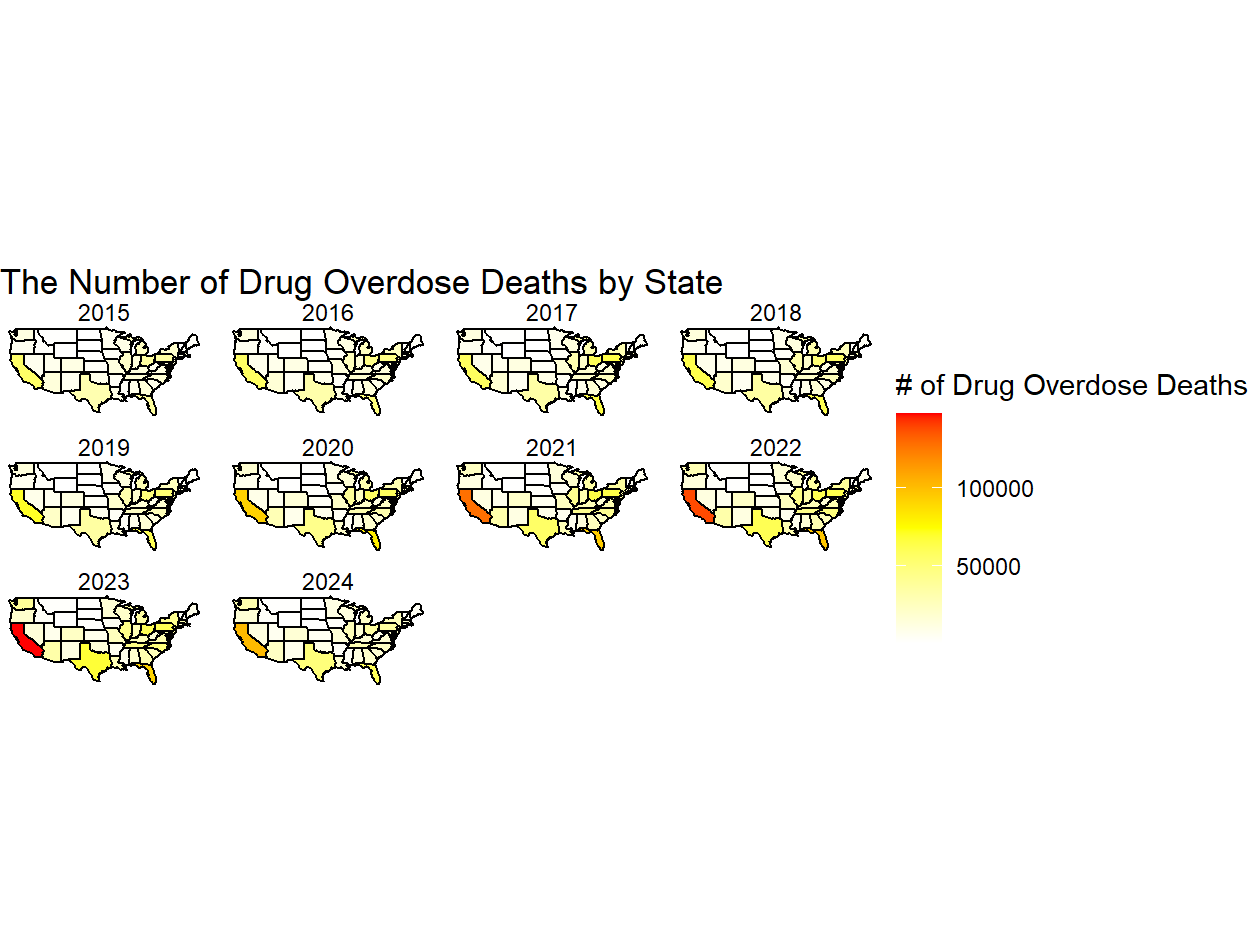
\includegraphics[width=1\linewidth]{PS6a_Hunt.png}
    \label{fig:enter-label}
    \end{figure}
\noindent Visualization B: 
\\This is a more classic line trend graph that showcases the total number of drug overdose deaths per drug type over time. This is a very practical visualization that helps highlight the overall trends while also allowing for comparison between different drug types. For instance, this graph shows that synthetic opioids are by far the largest contributor. I think trend line graphs like these are very useful, and knew I wanted to make one for this project.
\begin{figure}[H]
    \centering
    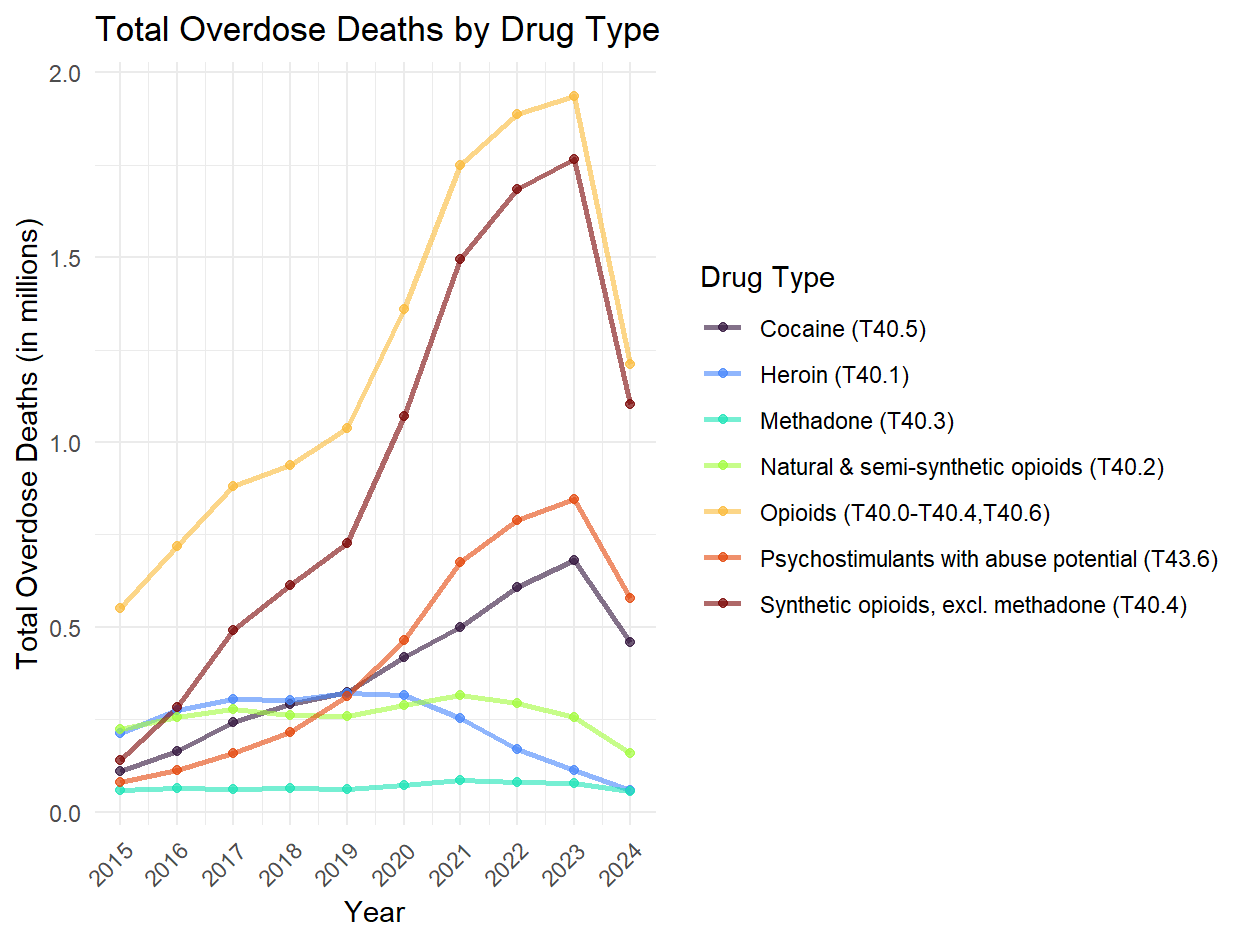
\includegraphics[width=1\linewidth]{PS6b_Hunt.png}
    \label{fig:enter-label}
    \end{figure}
\noindent Visualization C:
\\For the last visualization, I was inspired by the stacked area plot example given in the ggplot notes and wanted to replicate it with my data. In this instance, we see a stacked area plot that shows total overdose deaths over time in stacked proportions by month. This type of visualization lets you see the overall trend in the number of deaths per year, as well as the seasonal variation in the number of drug overdose deaths. In this case, we can see that there is no substantial seasonal variation. 
\begin{figure}[H]
    \centering
    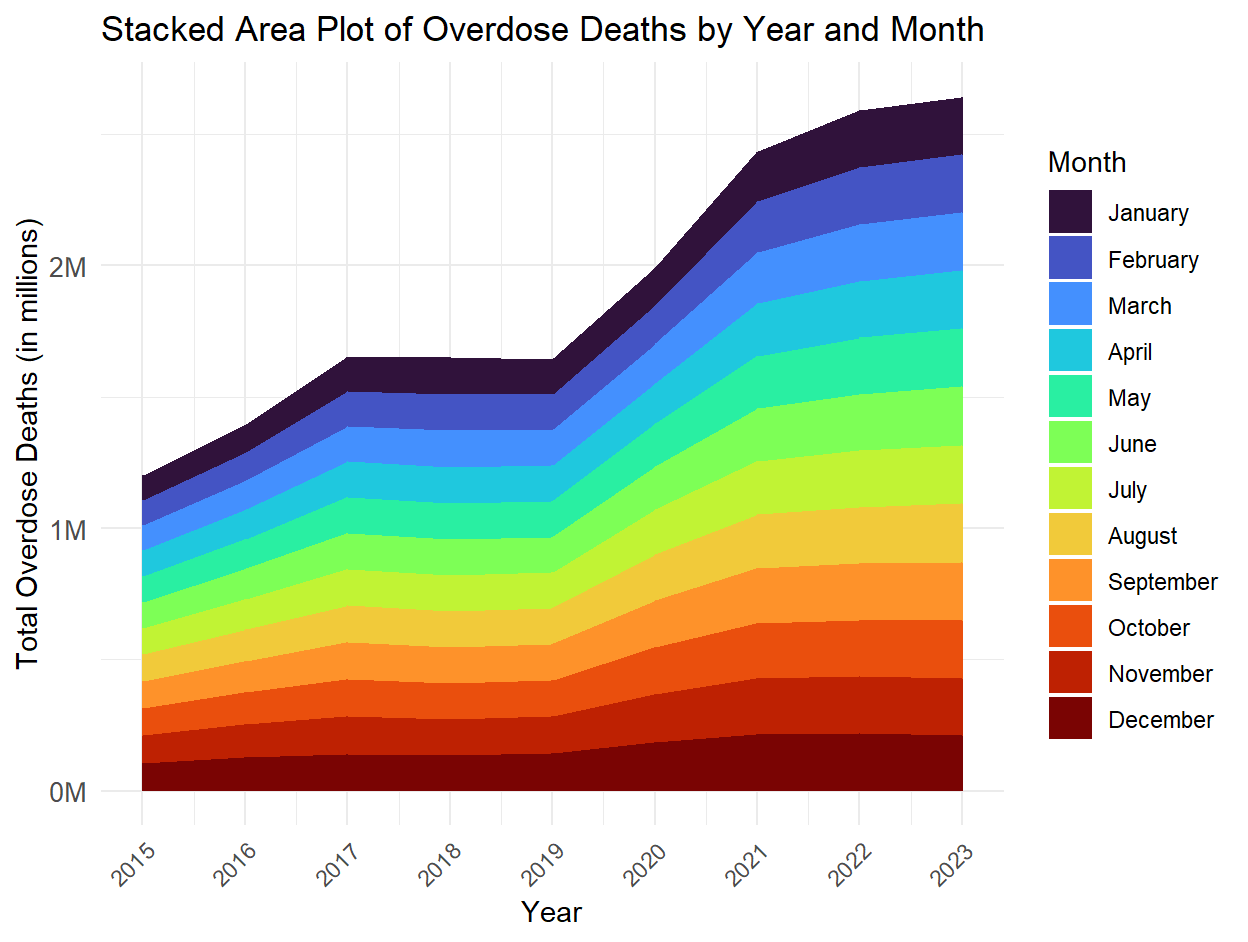
\includegraphics[width=1\linewidth]{PS6c_Hunt.png}
    \label{fig:enter-label}
    \end{figure}
\end{document}
